% \begin{savequote}[75mm]
% Nulla facilisi. In vel sem. Morbi id urna in diam dignissim feugiat. Proin molestie tortor eu velit. Aliquam erat volutpat. Nullam ultrices, diam tempus vulputate egestas, eros pede varius leo.
% \qauthor{Quoteauthor Lastname}
% \end{savequote}

\chapter{Object representations in lateral visual cortex}
\newthought{Shape is a diagnostic feature} of object identity. Visually similar objects, such as a pear and an apple, can be grouped together by certain shared visual features. On the other hand, different images or views of any one object can look dramatically dissimilar, yet still belong to the same object. The ventral visual pathway in the primate brain is thought to transform non-diagnostic, low-level representations of features that may be common to many different objects into high-level representations that are both diagnostic of object identity, or selective for a given object, and robust to variations in particular appearance, or tolerant to identity-preserving transformations. In the first chapter, we established the behavioral ability of rats to perform visual object recognition and quantified their perceptual choices of object similarity. We next turned our attention to the neuronal substrates of these abilities. 

% Neural subtrates of object recog. -- what do we know from primates.
Primate visual cortex is arranged hierarchically, with visual inputs from the thalamus first arriving in so-called ``striate'' cortex (also known as area V1), before being processed and forwarded through a successive chain of hierarchically-organized visual areas (area V2 > area V4 > inferotemporal cortex) curving along the ventral surface of the brain. Along each stage of the ventral stream, there is a gradual increase in object selectivity and tolerance, culminating in area IT, at the highest level of the ventral pathway. 

Several key trends have been observed in the response properties of visual neurons as one progresses from ``lower'' to ``higher'' visual areas along this ventral pathway. First, the region of visual space that a given cell responds to (the ``receptive field'') gradually increases as one moves along the ventral pathway, with receptive fields in the highest stages of visual cortex sometimes responding to up to half of the visual field\cite{OpDeBeeck2001}. Meanwhile, selectivity for complex object features also increases along the ventral visual pathway, with neurons in later stages of the pathway responding only to very particular configurations of features\cite{Desimone1984, Logothetis1996}. Critically, as one progresses along the ventral pathway, neurons also exhibit greater tolerance to identity-preserving transformation of the retinal image -- that is, neurons tend to retain their selectivity for particular object features even if those features are, for instance, moved around on the retina, or scaled up or down in size\cite{Ito1995}.These combined features of selectivity and tolerance are in many ways the key computational hallmarks of high-level vision\cite{DiCarlo2007, DiCarlo2012}. 

% Previous rodent studies
% \section{Lateral visual cortex exhibits some of the same core properties found in primates}
Anatomical studies have shown that the connectivity of rodent visual cortex observes a similar hierarchical pattern, with thalamic inputs arriving in an analogous striate area V1 in posterior of the brain, and then projecting ventrally to a series of interconnected extrastriate areas\cite{Coogan1993}. However, while these areas have been characterized anatomically, much less is known about their function. Most of what we know about rat visual cortex beyond V1 comes from single-unit, electrophysiology studies that have characterized response properties of neurons in the context of visual object recognition\cite{Tafazoli2017, Vermaercke2014, Vinken2014}. While these studies differ in a few points (see Conclusion), a few key trends have been observed. First, all studies to date report an increases in receptive field size from V1 to LM to LI and beyond\cite{Tafazoli2017}. This is consistent with studies of extrastriate cortex in mice\cite{Murgas2020, Siegle2021}. Second, though there is not yet a clear consensus, several rat studies report increased shape selectivity or shape discriminability for single-units in extrastriate cortex\cite{Tafazoli2017, Vermaercke2014, Vermaercke2015}. Finally, most studies report some degree of tolerance to identity-preserving transformations: single-units recorded in extrastriate cortex along these lateral areas maintain shape selectivity or discriminability across changes in position, size, or rotation\cite{Vermaercke2014, Tafazoli2017}.


Consistent with previous studies in rats, and what might be expected from a primate-like hierarchical organization, we observed increasing receptive field sizes in areas V1, LM, and LI (see Chapter 3). However, we also found asymmetries in visual field representations and motion tuning preferences that may be particular to rodent visual cortex, as these are some of the more fundamental visual processing observations that have been reported in recent studies of mouse visual cortex\cite{Liang2018, Sit2020, Murgas2020}. To determine the extent to which rat lateral visual cortex intrinsically exhibits properties thought to be important for spontaneous, as opposed to learned, object recognition behavior, we recorded from neural populations in awake, naive rats presented with a subset of the same stimuli used for the trained rats (see Chapter 1, Figure\ref{fig:behavior_generalization}) to probe axes of transformation in which object identity is either preserved or gradually morphed to a new identity across changes.

% ---------------------------------------------------------------
% Single neuron selectivity and tolerance
% ---------------------------------------------------------------
\section{Single neurons exhibit selectivity and tolerance}
\begin{figure}[t!]
    \includegraphics[width=\textwidth]{figures/chapter_4/fig_4-1_single_cell_selectivity_tolerance/fig_4-1_single_cell_selectivity_tolerance.pdf}
    \caption[Single neuron selectivity and tolerance]{Selectivity and tolerance. 
    \textbf{A.} Transformations tested: 5 stimulus sizes (identity-preserving) and 9 morph levels (identity-changing). 5 luminance stimuli (fullscreen) were matched for each size
    \textbf{B.} Rat visual areas in this study. 
    \textbf{C.} Morph selectivity (left) and size tolerance (right) for an example V1 FOV. Black lines, single cell tuning profiles. Color lines, example cells: Green, the first set of traces (middle). Purple, the lower set (bottom). Time courses arranged as in \textbf{A}. Lines and shading, mean and SEM across repeats.
    \textbf{D.} Same as \textbf{C}, but for an LM FOV.
    \textbf{E.} Same as \textbf{B} and \textbf{C}, but for an LI FOV.
    \textbf{F.} Distributions of size tolerance for V1, LM, and LI cells. Each dot is a cell, black lines denote mean and SD across cells.
    \textbf{G.} Same as \textbf{F}, but for morph selectivity. 
    \textbf{H.} Correlation between size tolerance and morph selectivity for example V1 (left), LM (middle), and LI (right) FOVs. Each dot is a cell. Line and shading, linear fit and 95\% CI.
    \label{fig:selectivity_tolerance}}
\end{figure}

One key feature of the primate ventral stream is a gradual increase in shape or object selectivity and a parallel increase in tolerance to identity-preserving transformations. Previous studies have shown that single-units in monkey IT exhibit a trade-of between these properties: neurons that are highly selective are less tolerant to identity-preserving transformations and highly tolerant neurons are not as selective to particular objects\cite{Zoccolan2007}.

To determine whether single neurons exhibited similar characteristics in rat visual areas, we first measured single neuron response profiles in areas V1, LM, and LI. For identity-changing transformations, we tested a subset of the morphs used to probe trained animals’ naive perceptual boundaries, and for identity-preserving transformations, we tested a subset of sizes covering the range of stimulus sizes used to test behavioral generalization to identity-preserving transformations (see Chapter 1, Figure\ref{fig:behavior_generalization}). Since size changes come with large changes in luminance, we also presented a subset of full-screen gray-scale stimuli that were luminance-matched to each size tested (Figure\ref{fig:selectivity_tolerance}A).


All areas contained a diverse range of object selective and size tolerant cells. For example, even in one V1 FOV, we found cells that exhibited clear size tuning without morph selectivity, morph tuning that was preserved across different sizes, as well as luminance-tuned cells that were also sensitive or insensitive to the different morphs and sizes. Overall, we found that across our object stimuli, cells in LI had the lowest lifetime sparseness, while cells in V1 and LM were similarly high in sparseness. Since the images varied in morph level and size, the sparseness observed in V1 and LM could reflect a higher selectivity for morph shapes or a lower tolerance for varying sizes. To quantify the amount of object selectivity and tolerance, we calculated a morph selectivity index (MX) and a size tolerance index (ST) for each cell\cite{Zoccolan2007}. We found a range of tuning profiles across cells that was comparable between the three areas (Figure\ref{fig:selectivity_tolerance}B-D). On average, we found that relative to V1 and LM, LI cells were both less selective to morphs and more tolerant to size (Figure\ref{fig:selectivity_tolerance}E-F). Notably, this difference was not attributable to overall lower response magnitudes in LI: although we found fewer LI cells selective or responsive to the object stimuli overall, of the cells that were responsive, response magnitudes were comparable across areas. 

It is possible that the relatively higher average morph selectivity in V1 and LM cells reflects greater sensitivity to overall luminance values. To characterize the extent to which size or morph tuning simply tracks luminance sensitivity, we calculate the correlation between each cell's size tuning curve and its tuning curve for the size-matched luminance stimuli. While there were indeed cells whose size- or morph-tuning profiles were tightly correlated with broad luminance levels, this was not the case for the majority of cells (V1: 9.8+/-6.8\% of cells with significant correlation between size and luminance tuning; LM: 12.6+/-8.2\%; Li: 12.2+/-9.1\%). 

To determine whether rat neurons exhibit a similar trade-off between shape selectivity and transformation tolerance, we calculated the correlation between morph selectivity and size tolerance for simultaneously recorded cells in each imaging site (Figure\ref{fig:selectivity_tolerance}H). We found a strong, negative correlation between morph selectivity and size tolerance for areas LM and LI. Notably, we also saw a negative correlation for V1 imaging sites, but to a weaker degree. To determine whether the strength of this trade-off differed between the three areas, we scrambled each cell’s selectivity index and tolerance index and compared correlation coefficients for those populations that passed the shuffle test (shuffle test, p<0.05 over 5000 iterations). We found that correlation coefficients for sites in areas LM and LI were significantly more negative than those in area V1. 

% A critical property of single neurons in IT is the preservation of rank-ordered object selectivity, that is, relative tuning preference for a set of objects is maintained across changes in identity-preserving transformations such as position or size\cite{Li2009, REFREF}. 

% ---------------------------------------------------------------
% Arousal
% ---------------------------------------------------------------
\section{Arousal modulates tuning properties} 
\begin{figure}[t!]
    \includegraphics[width=\textwidth]{figures/chapter_4/fig_4-2_arousal/fig_4-2_arousal.pdf}
    %\vspace{.1in}
    \caption[Arousal modulates tuning]{Arousal modulates tuning. 
    \textbf{A.} Example view of the face-tracking camera pointed at the animal’s face, overlaid with face feature annotations for whiskers and pupil tracking.
    \textbf{B.} Example pupil diameter trace (top) and neural responses (bottom) for repeated presentations of a single condition type. Gray bars in the middle show the stimulus period of each trial. Colormap shows z-scored responses.
    \textbf{C.} Response magnitude on trials in which animals were in “high” (magenta) and “low” (cyan) arousal states (i.e. trials with an average pupil diameter above or below the 67th and 33rd percentiles, respectively). Points, average response magnitude across cells of a given imaging site. Error bars, SD.
    \textbf{D.} Size tolerance as a function of arousal state, for each visual area. Points, average response magnitude across cells of a given imaging site. Horizontal bars, average across sites for a given visual area. Error bars, SD.
    \textbf{E.} Morph selectivity as a function of arousal state, for each visual area. Notation as in \textbf{E}.
    \textbf{F.} Correlation coefficient for morph selectivity versus size tolerance as a function of arousal state, for each visual area. Notation as in \textbf{E}, \textbf{F}.
    \label{fig:arousal}}
\end{figure}

Since the animals were head-fixed and awake, we were able to monitor their face movements and other behaviors during imaging sessions. Face video was acquired simultaneously and synced with neural acquisition (Figure\ref{fig:arousal}A-B). Arousal states modulate both single neuron tuning and population decodability. We do not know how population representations supporting object recognition change across different arousal states. Trials were separated into ``high'' or ``low'' states by pupil size, and we compared single unit metrics of size tolerance and shape selectivity as well as linear separability of population representations across areas V1, LM and LI. Consistent with previous studies of arousal modulation in V1, we found that response magnitudes were greater when the animal was in a high arousal state, as compared to a low arousal state, and this was also true for areas LM and LI (Figure\ref{fig:arousal}C). Across these visual areas, shape selectivity was also greater and size tolerance was lower in high arousal compared to low arousal states (Figure\ref{fig:arousal}D-E). However, in V1, but not in LM and LI, the strength of this relationship, as measured by the correlation coefficient between size tolerance and morph selectivity, was weaker in high arousal states (Figure\ref{fig:arousal}F). These results suggest a possible decoupling between selectivity and tolerance in V1 populations, in that the trade-off between selectivity and tolerance appears less affected by arousal states at the single neuron level.


% ---------------------------------------------------------------
% Morphs
% ---------------------------------------------------------------
\section{Single cells show object discriminability}
% Morphs -- neurometric curves, single-neuron disriminability

Given the range of shape selectivity and size tolerance we observed in single cells across areas V1, LM, and LI, we next determined the extent to which cells could discriminate object identity for the two anchor objects. When we tested the trained rats (Chapter 1), we first trained them to correctly recognize object A from object B, and rats had to pass a criterion performance level of at least 70\% accuracy --- only rats that demonstrated clear discrimination performance were included in tests of perceptual similarity along the morph continuum. However, since the rats we imaged here were not trained, the anchor objects did not have any particular meaning: it is not necessarily the case that cells should faithfully track the shape continuum from one anchor extreme to the other. Rather, a cell could selectively prefer one of the intermediate morphs (for example, the green cell shown under LI in Figure\ref{fig:selectivity_tolerance}E). 

\begin{figure}[t!]
    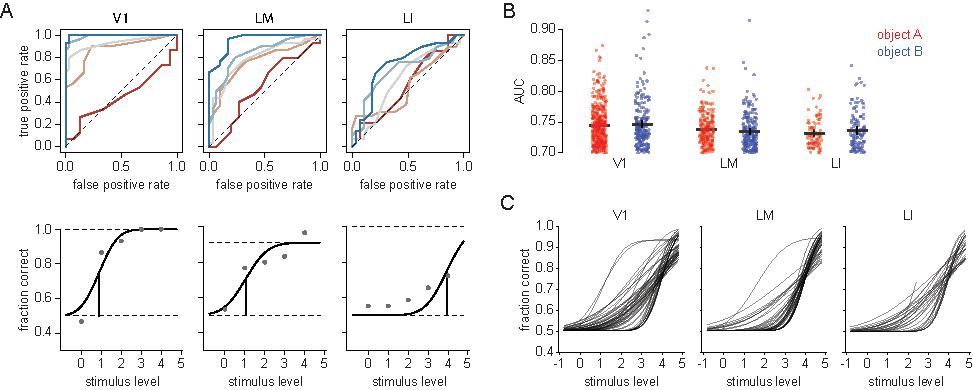
\includegraphics[width=\textwidth]{figures/chapter_4/fig_4-3_neurometric/fig_4-3_neurometric.pdf}
    %\vspace{.1in}
    \caption[Single neuron discriminability]{Single neuron discriminability. 
    \textbf{A.} Distribution of discriminability (AUC) for cells selective for either object A (red) or object B (blue), which were the two anchor objects.
    \textbf{B.} \textit{Top}, Example time courses at each morph level at the preferred size for a cell preferring object B. \textit{Bottom}, Example time courses for a cell preferring object A. Horizontal bar, stimulus period. 
    \textbf{C.} \textit{Top}: Example ROC curves for the cell shown in \textbf{B}, \textit{top}. The area under these curves (AUC) measures how well a neuron discriminates one image, the preferred object B, from each other image, or the other morph levels. Red corresponds to object A (morph level 0\%B) and blue corresponds to object B (morph level 100\%B). \textit{Bottom}: ROC curves, but for the cell shown in \textbf{B}, \textit{bottom}. 
    \textbf{D.} \textit{Top}: Corresponding neurometric curves fit to the AUC values at each morph level for the cell shown in the top panels of \textbf{B} and \textbf{C}. \textit{Bottom}: Corresponding neurometric cures for the cell shown in the bottom panels of \textbf{B} and \textbf{C}. 
    \textbf{E.} Neurometric curves for all selective, well-fit cells in V1 (left), LM (middle), and LI (right). Only cells that passed criterion performance (70\% accuracy) were tested on the intermediate morphs, then fit for their ability to discriminate the objects as a function of morph level. Thin gray lines correspond to individual cells. Red, mean and SD across cells preferring object A. Blue, mean and SD across cells preferring object B.
    \label{fig:neurometric}}
\end{figure}

% \begin{figure}[t!]
%     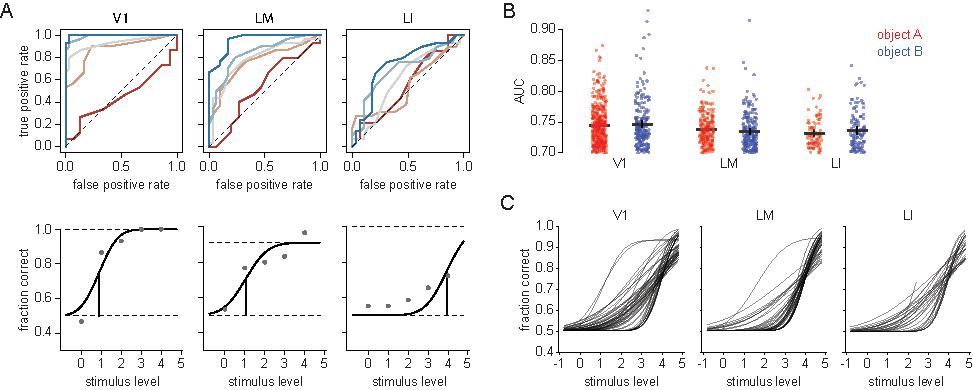
\includegraphics[width=\textwidth]{figures/chapter_4/fig_4-3_neurometric/fig_4-3_neurometric.pdf}
%     %\vspace{.1in}
%     \caption[Single neuron discriminability]{Single neuron discriminability. 
%     \textbf{A.} Top, Example ROC curves for an example cell in V1 (left), LM (middle), and LI (right). The area under these curves (AUC) measures how well a neuron discriminates object A from object B as a function of stimulus level, which is the difference between the morphs. Level 0 (red) corresponds to the lowest morph difference, the middle morph (equal parts A/B), while the highest level (blue) corresponds to the highest morph difference, or 0\%B versus 100\%B, which just is 100\%A and 100\%B. Bottom, Corresponding neurometric curves fit to the AUC values at each stimulus level. At the highest stimulus level, the morphs are maximally different, and so the fraction of ``correct'' responses are greater. Vertical lines indicate the level at which performance was at 75\%.
%     \textbf{B.} Distribution of discriminability (AUC) for cells selective for either object A (red) or object B (blue), which were the two anchor objects.
%     \textbf{C.} Neurometric fits for the best cells in V1 (left), LM (middle), and LI (right). Only cells that passed criterion performance (70\% accuracy) were tested and fit for their ability to discriminate the objects as a function of morph level.
%     \label{fig:neurometric}}
% \end{figure}


% To determine the extent to which cells can discriminate the original anchor objects, similar to the way we trained the behaving rats to do so, we selected a subset of cells that did exhibit selectivity to one anchor over the other (see Methods). Specifically, we measured neural performance on the object discrimination task as the neuron's ability to distinguish object A from object B at each level of morph (Figure\ref{fig:neurometric}A). At the lowest level, the morph level is 50\%A and 50\%B, and so the two objects to be discriminated are equally A and equally B, and thus, discriminability should be at chance. From 0, morph differences increase, \textit{e.g.}, from 40/60 to 30/70, and so on, until the maximum level difference, 0/100, which just is the original anchor objects A and B (i.e., 0\%B is 100\%A, and vice versa). For each neuron, we quantified the degree of overlap between its responses to two alternatives with a receiver operating characteristic (ROC) analysis \cite{Britten1992, Rust2010SelectivityIT}. For example, given an image that is 30\%B (alternative 1) and one that is 70\%B (alternative 2), we generated an ROC curve by computing the proportion of trials for alternative 1 on which the cell's response exceeded the criterion versus the proportion of trials for alternative 2 on which the response exceeded the criterion, for a range of criteria. The AUC is then taken as the area under this curve. The curve is calculated for each stimulus level, and the AUCs under each of these curves are then fit with a neurometric curve. 

Overall, there were fewer cells in LI that were strongly selective to one anchor or the other, relative to V1 or LM (Figure\ref{fig:neurometric}B). However, of those that were selective, average discrimination performance was comparable across visual areas. In all cells for which we were able to fit neurometric curves (Figure\ref{fig:neurometric}C), most were biased toward the stimulus level of maximum difference between the two objects. This was expected to some degree, as only cells that were successful at discriminating objects at that level (max level means 100\%A and 100\%B). Although these results cannot be interpreted in the context of train rats, for whom these objects would have behavioral significance, they serve to demonstrate that single neurons in each visual area are highly capable of discriminating the two objects, and those that do follow a predictable response profile (the more different A and B were, the easier it was for the neuron to discriminate them).  


% ---------------------------------------------------------------
% Population responses
% ---------------------------------------------------------------
\section{Population responses are linearly separable}
How the brain achieves the critical combination of high object selectivity with high tolerance to particular views remains a mystery. It is thought that each successive stage of the ventral stream computes a series of operations that make object representations increasingly linearly separable. In our behavior experiments, rats accurately classified novel image transformations in the absence of any feedback, suggesting explicit training is not required for generalization behavior (see Figure\ref{fig:behavior_generalization}). The single neuron response properties in our naive rats suggest that rat visual cortex may have some of the important features considered to be important for tolerant visual object representations.


\begin{figure}[t!]
    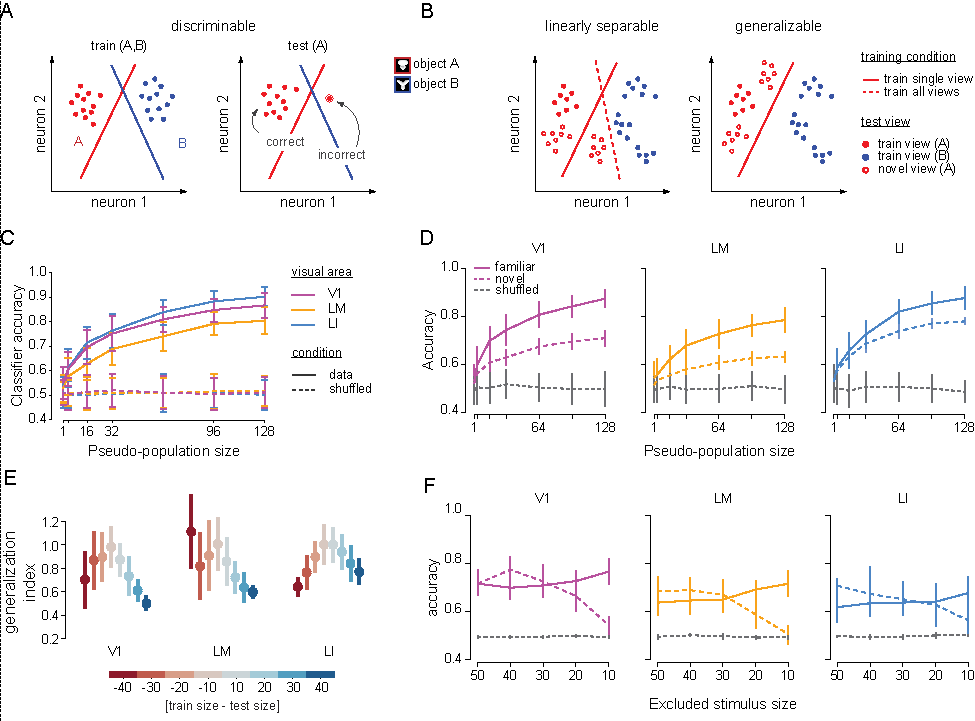
\includegraphics[width=\textwidth]{figures/chapter_4/fig_4-4_neural_generalization/fig_4-4_neural_generalization.pdf}
    \vspace{.1in}
    \caption[Population representations of objects]{Linear separability and tolerance. 
    \textbf{A.} Test schematics (adapted from \cite{Rust2010SelectivityIT}). A hypothetical population response for 1 presentation of an image as a point in N-dimensional space (N=number of neurons). Different trials of the same image (blue) form a cloud in this N-D space. The ability of the population to discriminate the images is proportional to how far apart the response clouds are. Linear classifier approaches identify the optimal hyperplane that separates one image (blue) from the other (green). Performance is measured as the proportion of times that response vectors fall on the correct side of the hyperplane. 
    \textbf{B.} \textit{Left}: A population that supports generalization under one test (dashed) but fails under another (solid) for different views (blue clouds) of an object. \textit{Right}: A population that passes tests of generalization when testing on a single training condition (solid line in \textit{left}).
    \textbf{C.} Linear separability as a function of population size (see \textbf{B}, left) for V1, LM, and LI. Classifiers were trained on with responses from all sizes. Dotted, shuffled labels. Error bars, bootstrapped estimates of the 95\% CI of the mean accuracy. 
    \textbf{D.} Generalization test accuracy (see \textbf{B}, right) by population size for V1 (left), LM (middle), and LI (right). Classifiers were trained at 1 stimulus size, then tested on new samples of the same (black) or novel stimulus sizes (blue). Dotted lines and error bars as in \textbf{C}.
    \textbf{D.} Generalization score (ratio of novel to trained) split by the difference between train and test stimulus sizes (N=128 cells).
    \textbf{E.} Generalization test accuracy at each trained stimulus size. Classifiers were trained with 4 out of 5 stimulus sizes, then tested on different trials of the training size (black) or on new trials of the held-out, novel size (blue), for all combinations of train/test sizes. Error bars, SD across imaging sites. Dotted lines, shuffled labels.
    \label{fig:neural_generalization}}
\end{figure}


However, during behavior, the animal has access to much more than the activity of a single neuron. To determine the extent to which neural populations in rat visual cortex are inherently capable of representations that support discrimination and generalization, we took a population-based approach to compare areas V1, LM, and LI in awake, but untrained rats. Specifically, we trained linear SVMs with neural responses to these same object images to classify the responses as belonging to object A or object B \cite{Hung2005, Li2009, Rust2010SelectivityIT}. We then tested the classifiers on each of the two types of generalization tasks performed by the trained rats. 

Before testing the ability of each population to generalize across identity-preserving transformations, we first tested how well the objects could be discriminated from each other at each of the tested transformations. That is, if a given population failed to discriminate the objects at a given size, failure to generalize to that size would be trivial. For each imaging site, or set of simultaneously recorded cells, in each visual area, we trained linear classifiers to discriminate the two objects at each size, then scored accuracy on trials of the same condition that the classifier had never seen. To avoid trivial generalization due to poor baseline performance, only those populations with average test accuracies greater than accuracies calculated from shuffled object labels were included. 

To test discriminability of the two anchor objects, we first tested neural representations under a ``Train 1, test same'' regime: At each stimulus size tested, we trained classifiers to discriminate object A from object B. Overall, discrimination accuracy improved with increasingly larger stimulus sizes. This is consistent with previous single-unit studies of aggregated populations, though here we report performance for simultaneously recorded populations. This stimulus size dependence was present in all visual areas, and notably, overall performance was comparable across areas, as well. Specifically, average test scores were similar for populations in V1, LM, and LI, with mean scores in V1 and LM being slightly higher, but not significantly different, than LI (mean accuracy +/- std: V1, 0.73 +/- 0.08, n=9 sites; Lm: 0.68 +/- 0.04, n=5 sites; Li: -0.64 +/- 0.09, n=4 sites; Mann-Whitney U test, p>0.05 corrected for multiple comparisons). As expected, we also found better discrimination accuracy for larger neural population sizes. Only imaging sites that passed this baseline discrimination task were included in further tests of generalization performance (see Methods). 

% Linear separability.
To quantify linear separability, we trained linear classifiers (support vector machines) to discriminate the two original objects from the neural responses in each area across different training regimes. The linear-readout scheme is important in that it is a simple, biologically plausible processing step that amounts to a thresholded sum taken over weighted synapses. This classifier approach does not provide a measure for the total information present in the population, but rather estimates the lower bound on the information explicitly accessible to the population to support the visual task. 

We started with a ``Train all, test all'' scheme:  Classifiers were first trained to discriminate object A from object B across all stimulus conditions, then tested on new samples of object A and object B. This is a measure of how separable object representations are across the different stimulus sizes. We found that classifier accuracy was comparable across areas V1, LM, anbd LI for all population sizes (Figure\ref{fig:neural_generalization}B). % OVERLAP RFS?

% Arousal
% Increased shape selectivity could result in better linear separability, but decreased size tolerance could result in worse linear separability. REFREF.
% Arousal
% Consistent with the above results, we also found that linear separability of object representations was improved in high arousal states for V1, but was unaffected in LI, despite all areas exhibiting shifts in tolerance and selectivity in the same directions. However, LM also exhibited improved linear separability in high arousal states, like V1, despite there being no significant change in the linear relationship between selectivity and tolerance. This suggests that the tolerance/selectivity tradeoff may differentially affect object encoding and readout across visual areas.

Based on the performance of our trained rats, we know that behaving animals achieve high levels of accuracy on completely novel, never-before-seen views of objects (see Figure\ref{fig:behavior_generalization}). To determine whether this might be true even in naive, untrained animals, we conducted a second test of generalization. Generalization to completely novel stimulus conditions was called the “Train 1, test each of the others” scheme:  We trained classifiers to discriminate object A from B at one stimulus size, then tested how well they generalized to each of the other, novel stimulus sizes. For example, if we test on stimulus size 10, the test cases were 1 “trained” condition (different samples of stimulus size 10), and 4 “novel” conditions (the 4 other stimulus sizes that the classifier never saw). We observed accuracies well above chance for all visual areas, with overall accuracies improving for larger population sizes (Figure\ref{fig:neural_generalization}C). 
Notably, the gap between accuracy for trained and novel conditions was smaller for LI, compare to V1 and LM. Given the earlier observation that single cells in LI exhibited a slightly higher size tolerance, we asked whether generalization performance was dependent on which stimulus sizes the classifiers had access to in training. Trivially, generalization might be better if the difference in training and testing conditions is small: training to discriminate object A from B at stimulus size 10 might result in better generalization to stimulus size 20, compared to generalization to stimulus size 50. For each visual area, we calculated a generalization score, defined as the ratio of accuracy on trained conditions versus novel conditions. Since a high generalization score is trivially possibly for poor performance on both trained and novel conditions, we calculated this metric only for the largest, that is, best-performing population sizes for each visual area (n=128 cells). As expected, we found that generalization was best for training-testing regimes in which the difference in conditions was the smallest (Figure\ref{fig:neural_generalization}D). Interestingly, we found a slight asymmetry in that generalization was slightly worse if the novel stimulus size at test was smaller than the trained stimulus size, but only for V1 and LM. Generalization was symmetric about the difference between trained and novel conditions for LI.

To determine the extent to which generalization is facilitated by the composition of stimulus conditions on which the classifier trains, we trained and tested linear classifiers for each visual area using all combinations of stimulus sizes. Specifically, we used a ``Train a subset, test 1 other'' scheme:  Each classifier was trained to discriminate object A from B using a range of stimulus sizes, namely all but 1 of the stimulus sizes, then tested on its ability to generalize to the remaining stimulus size. We found that while LI was robust to different training-testing combinations, V1 and LM were specifically sensitive to novel sizes if it was smaller than the trained stimulus sizes (Figure\ref{fig:neural_generalization}E, Wilcoxon signed-rank test, p<0.01). 


% Discussion. 
\section{Concluding Remarks}

